\section{Cyclone III FPGA}
The FPGA used on this oscilloscope is Altera's Cyclone III EP3C25Q240 FPGA, with close to $25,000$ logic elements. After setting up the chip properly, it can be configured into countless different logic circuits based on the application needs. This is very useful in applications where high speed is important (for example, in taking samples for an oscilloscope), but the quantities that would be produced are too low for ASICs to make sense.

To set up the FPGA for some simple logic circuit, it must be programmed on power-up, either via JTAG or some configuration circuit/chip (the FPGA's memory is volatile, so it requires reprogramming every time it's powered back on). There are a number of ways to create the design for the FPGA logic. One way is to create straight-up VHDL. Another is to create a block diagram file and draw out the logic circuits that way.

Altera provides a piece of software called ``Quartus,'' which manages these different ways of designing the FPGA hardware connections. Quartus in fact provides a number modules that can be placed in a block diagram file. For example (and of particular use to us), a dual-clock FIFO can be placed in a design effortlessly. After creating a design, it can be programmed onto the FPGA.

\begin{figure}[ht!]
    \centering
    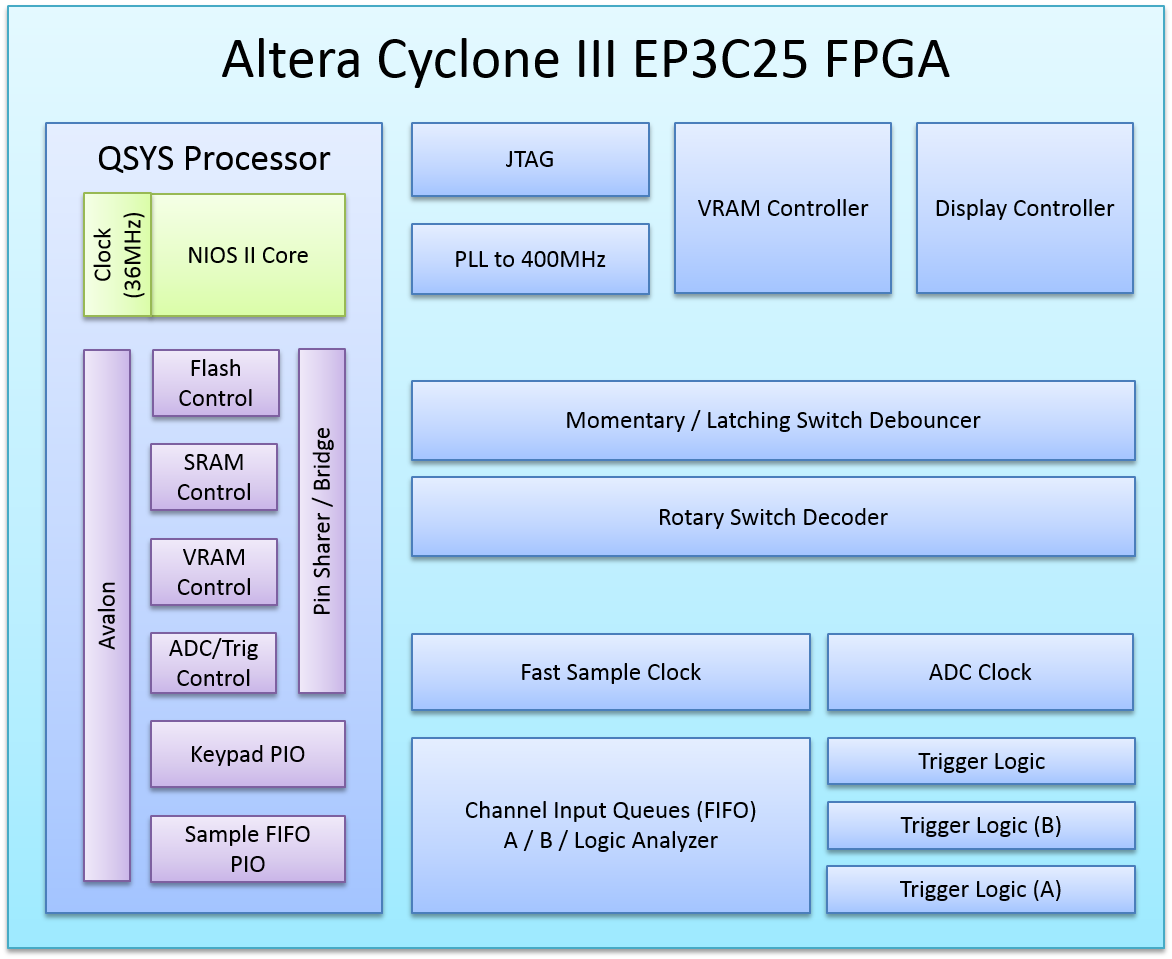
\includegraphics[width=3in]{block_diagrams/fpga.png}
		\caption{FPGA main components}
\end{figure}

Here's the major components of the FPGA logic. Most broadly, we have a NIOS II CPU, various clocks and timers, VRAM and display controllers, key debouncers and rotary encoder decoders, and finally, the scope sampling logic (FIFO storage, triggering, etc). We'll consider each of these in more detail.

\section{Clocks}

The system is fed an external $36MHz$ signal. This signal feeds direcly into some of the core logic, such as the NIOS II processor. However, in some cases we need a much faster (for sampling) or slower (for human-time-scale delays) clock signal.

\begin{figure}[ht!]
    \centering
    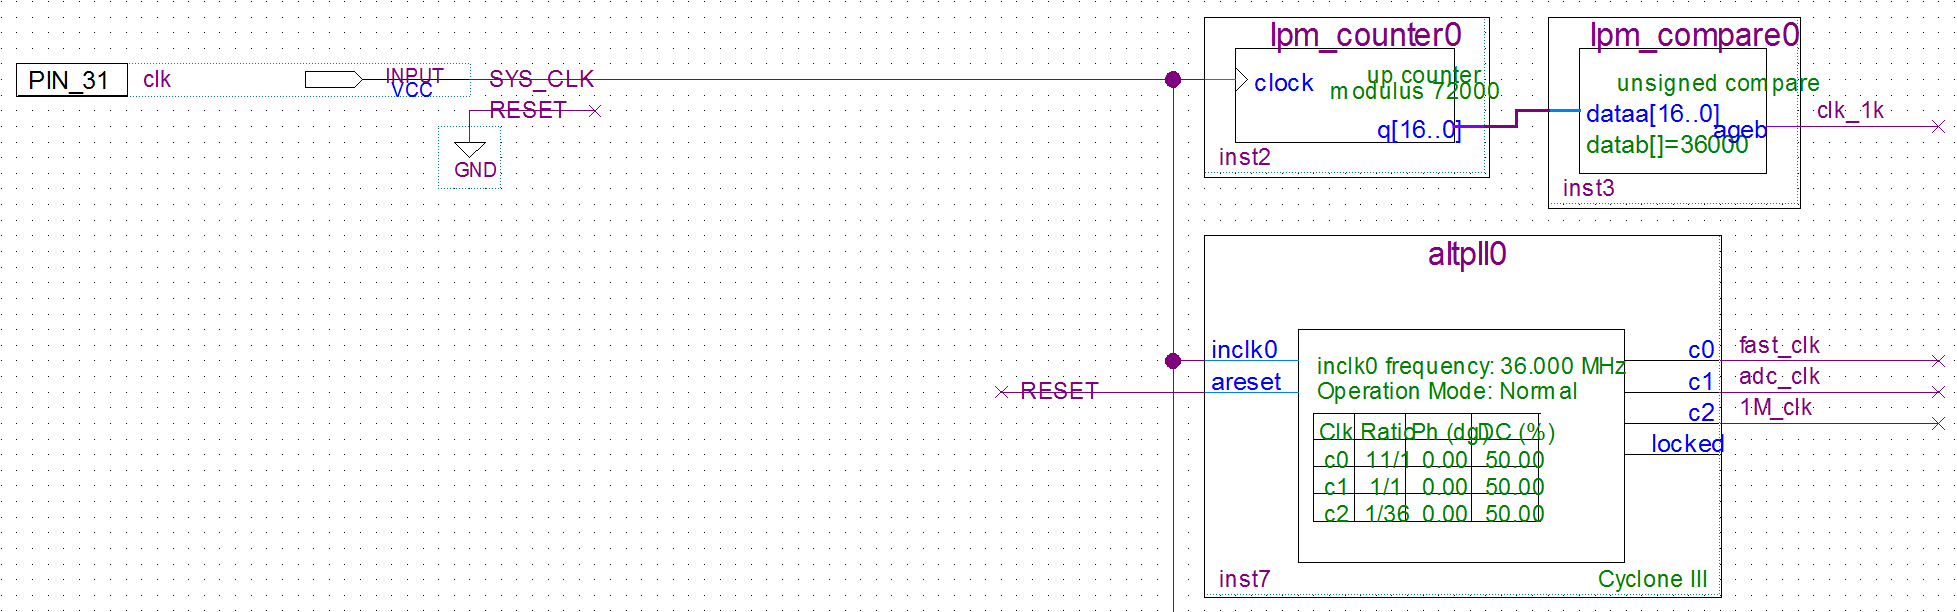
\includegraphics[width=6in]{fpga_logic/clocks.png}
		\caption{FPGA main clocks}
\end{figure}

A $50\%$ duty cycle $500Hz$ clock (incorrectly named \verb=clk_1k=) is produced by hooking a joint counter/compare to the $36Mhz$ signal. With a counter taken modulo $72,000$, incrementing at $36Mhz$ takes $2ms$. With a compare at $36,000$, we can then get a $50\%$ duty cycle $500Hz$ clock.

For the ADC and FIFO sampling, we want a much higher rate of about $400MHz$ (this is useful for the logic analyzer, even though the ADC can only produce new samples at $80MHz$). To do this, we use an phase-locked loop with an $11\times$ multiplier. This produces a $396MHz$ signal, close enough to $400MHz$. $400MHz$ was chosen because of its easy divisibility by factors of $2$ and $5$ (the common time scale factors used in scopes).

\begin{figure}[ht!]
    \centering
    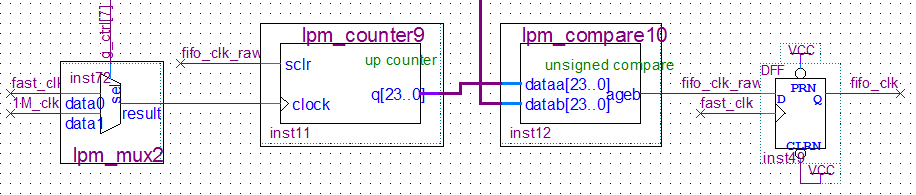
\includegraphics[width=6in]{fpga_logic/adc_sample_clk.png}
		\caption{FPGA sample clock}
\end{figure}

We need to be able to modify the rate at which we sample data in our code. To do this, we can attach a counter/compare to the fast $400MHz$ clock, and have the compare value set by the code. The logic above produces the sample clock. Notice that there are two selectable inputs to the counter/compre logic. One is the fast $400MHz$ clock for very high sample rates, and the other is a much slower $1MHz$ clock for slower sample rates. This is necessary because the $400MHz$ clock is less stable, especially with large counters such as a $32-bit$ counter, but has okay operating characteristics with the 24-bit one seen above.

\section{Sample Handling}

\begin{figure}[ht!]
    \centering
    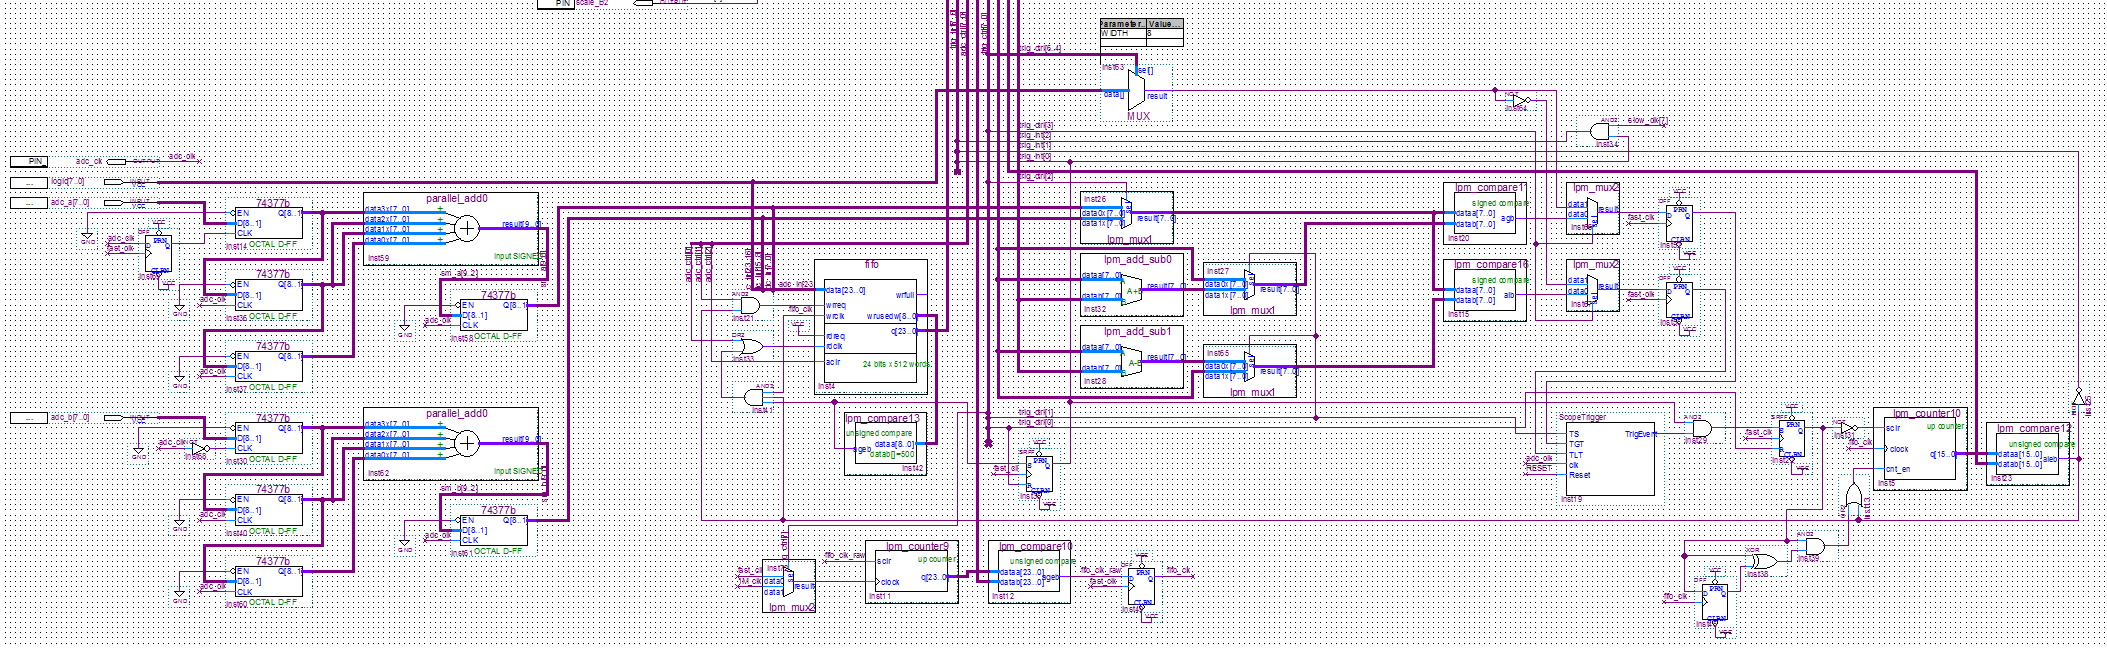
\includegraphics[width=6in]{fpga_logic/adc_overview.png}
		\caption{FPGA overview of scope sample handling}
\end{figure}

From left to right, we have the analog input logic, the sample FIFO and FIFO clock, and the trigger logic. We will look at each of these in detail.

\subsection{Analog Input}

The signal coming in from the ADC is somewhat noisy due to the suboptimal single-ended design of the analog frontend input to the ADC (it's designed for dual-ended input). Because of that, the signal can be a little noisy. To remedy this issue, the ADC signal is sent through a series of three 8-bit DFFs, and then a very simple 1D time-domain Gaussian blur is done on the signal.

\begin{figure}[ht!]
    \centering
    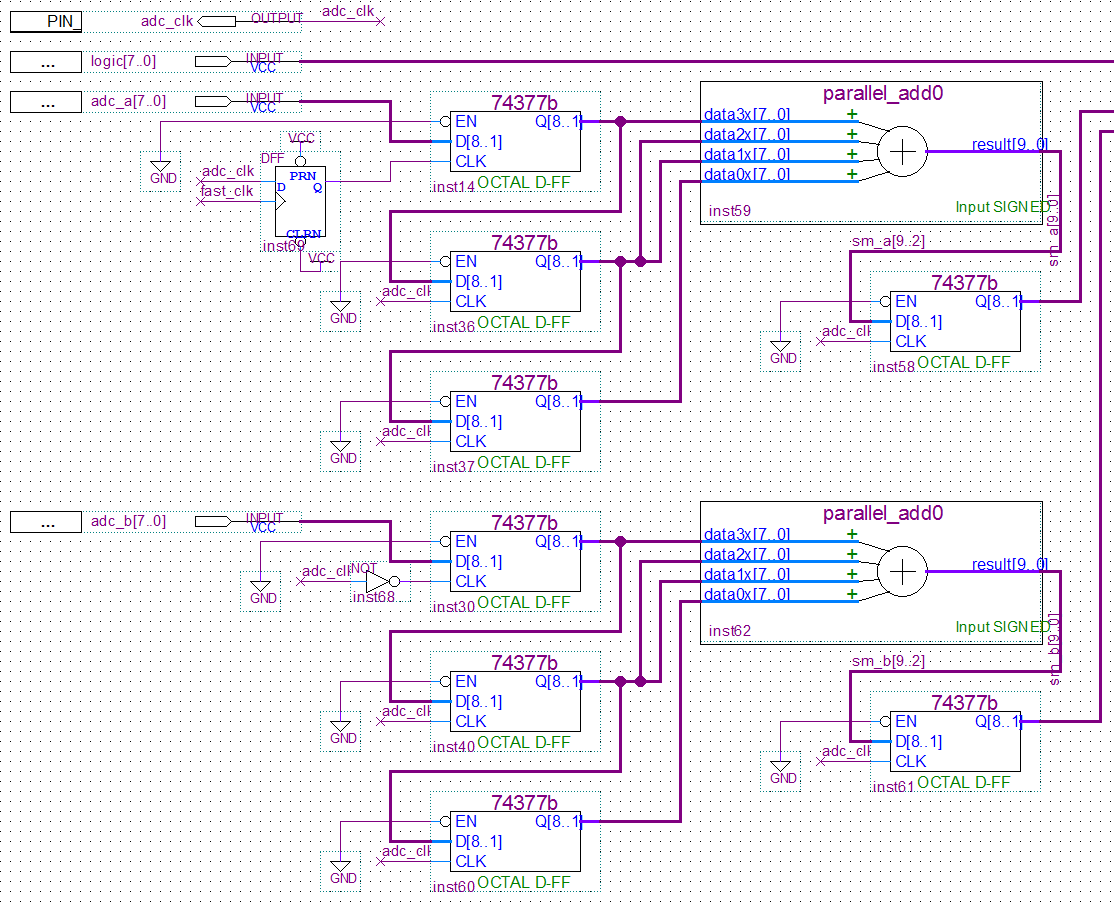
\includegraphics[width=5in]{fpga_logic/adc_input.png}
		\caption{FPGA sample input}
\end{figure}

Also notice that the first DFFs taking the ADC signal are offset by close to $180^o$ (in the top, there's a $\approx 2.5ns$ delay and in the bottom, a $\approx 12ns$ delay from the adc clock signal). This is because of how the ADC synchronizes its A and B channel outputs.

Output from the result of this logic is fed into the sample FIFO as well as the trigger logic.

\subsection{FIFO Sampling}

\begin{figure}[ht!]
    \centering
    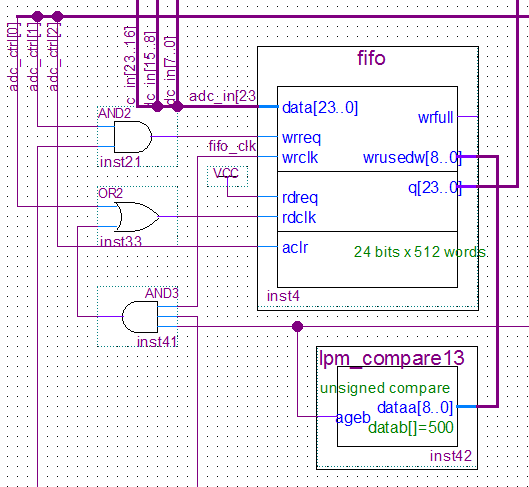
\includegraphics[width=2.5in]{fpga_logic/adc_fifo.png}
		\caption{FPGA sample FIFO}
\end{figure}

We are using a dual-clock FIFO in which data can be asynchronously written to (the back of the FIFO) and read from (the front of the FIFO) with different clocks. The way it's set up, the FIFO's write clock is based on the sample clock which can be as high as $400MHz$. Meanwhile, the read clock is bit-banged by the CPU when it wants to get the next 24 bits of data.

The FIFO logic is slightly complicated. First, when the FIFO fills, \verb=lpm_compare13= tells it to automatically start removing data (this allows the FIFO to act like a rotating buffer, always containing the last $N$ samples). Second, the FIFO stops collecting data automatically only when it sees a trigger event. Finally, the CPU has control over whether to allow reading and writing, and it can also clear the FIFO.

\subsection{Triggering}

\begin{figure}[ht!]
    \centering
    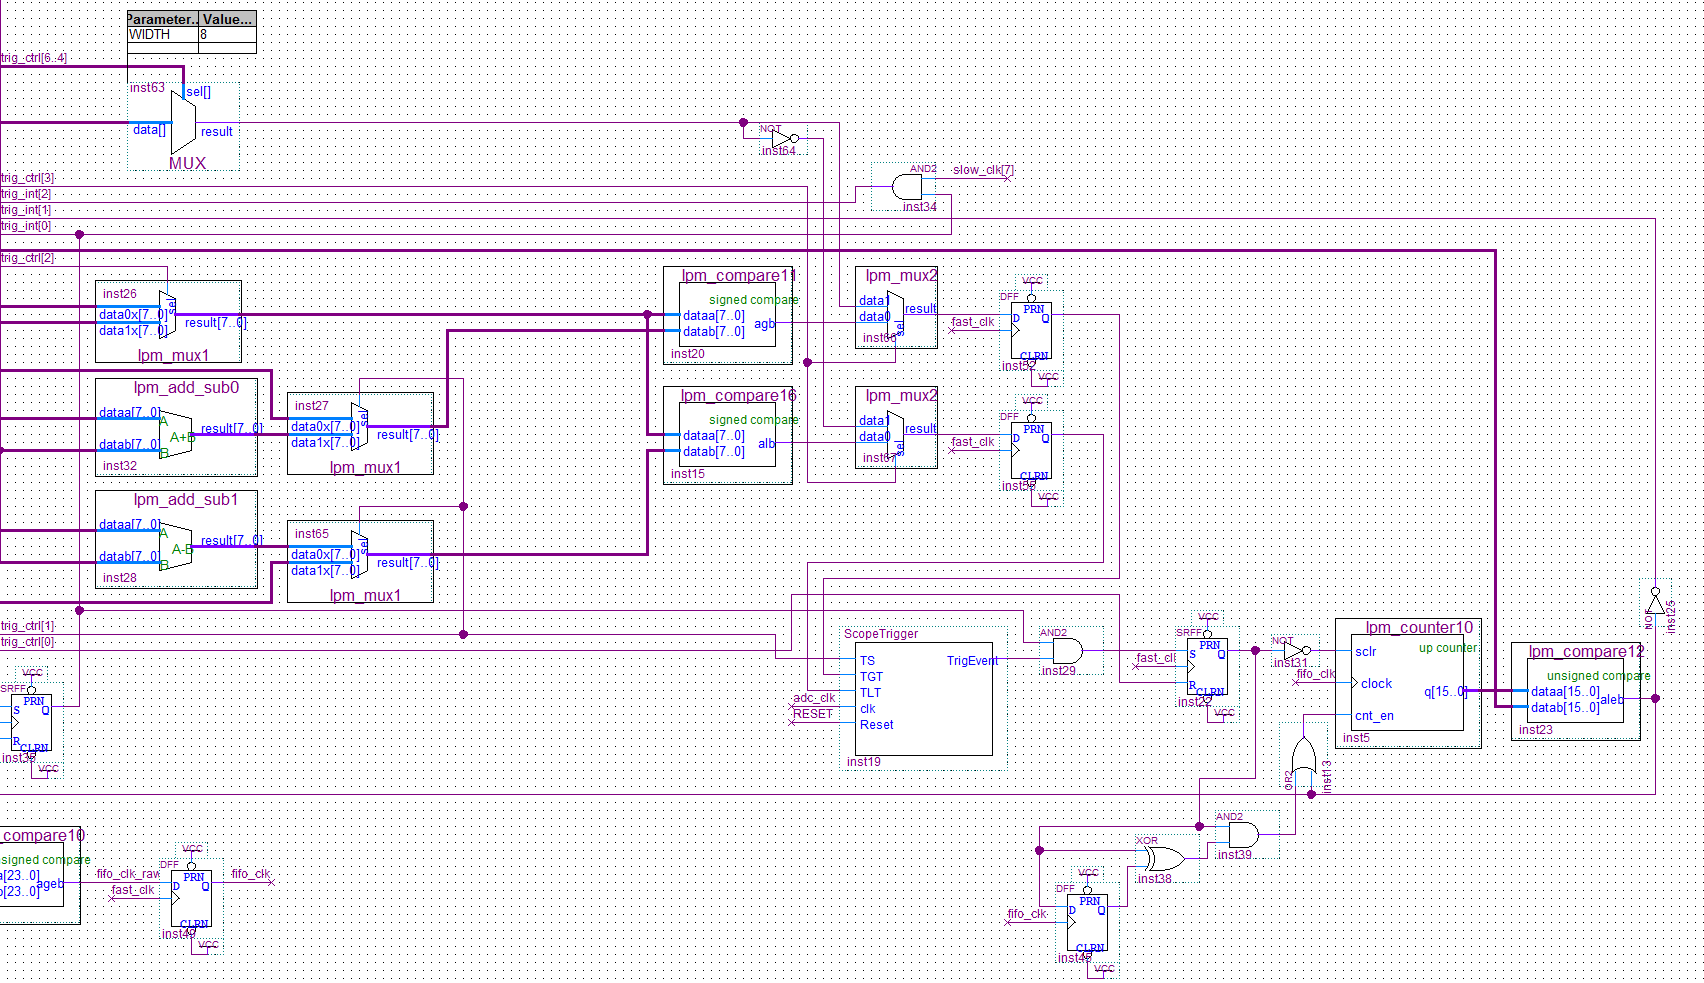
\includegraphics[width=6in]{fpga_logic/adc_trig.png}
		\caption{FPGA triggering}
\end{figure}

The function of this logic is to take the sample inputs and detect, using FPGA logic, when a given one of their values crosses a certain threshold, either in the positive or negative direction. This causes a trigger event which can automatically stop the sample FIFO after some specified delay. From here, the FPGA no longer accepts samples from the ADC or logic analyzer and the CPU can collect the FIFO samples. Once the CPU is finished, it can reset the FPGA logic to detect the next trigger event. The CPU provides information such as trigger channel, trigger level, trigger slope, and trigger error signals to control this section. It also provides a reset signal for when it's finished with the current trigger and wants the next one.

In the top left is a couple adders and MUXs. These take the desired trigger level and trigger error and produce dual outputs of the trigger level $\pm$ the trigger error. These outputs serve as upper and lower comparisons for the analog signal that's fed in through \verb=lpm_mux1= (which selects which analog channel to trigger on).

Above that is the logic analyzer input which also goes through a MUX to determine which bit (if any) to trigger on. From here, the compare results from \verb=lpm_compare11= and \verb=lpm_compare16= are MUXed with the logic analyzer and its inverse to select which of these signals we're interested in triggering against. Note that just as the analog signal has a lower and upper threshold, the logic analyzer can be fed as an upper threshold and the inverse of it as a lower threshold to provide identical thresholding functionality without requiring too much extra logic.

The selected trigger signals are cleaned with a DFF and then sent to the scope trigger state machine block which handles when to assert a trigger event based on the trigger thresholds \verb=TGT= and \verb=TLT= it sees, as well as the slope \verb=TS=. Once a trigger event is asserted, it sets an SRFF \verb=inst22=, which turns on counter \verb=lpm_counter10=. The logic below just turns off the counter before it loops over. This counter is responsible for the trigger delay, fed in by the CPU as a compare value for \verb=lpm_compare12=. Once the delay is over, the compare block outputs a high signal which sends an interrupt to the CPU and tells the FIFO to stop sampling data.

\subsection{Trigger State Machine}

\begin{figure}[ht!]
    \centering
    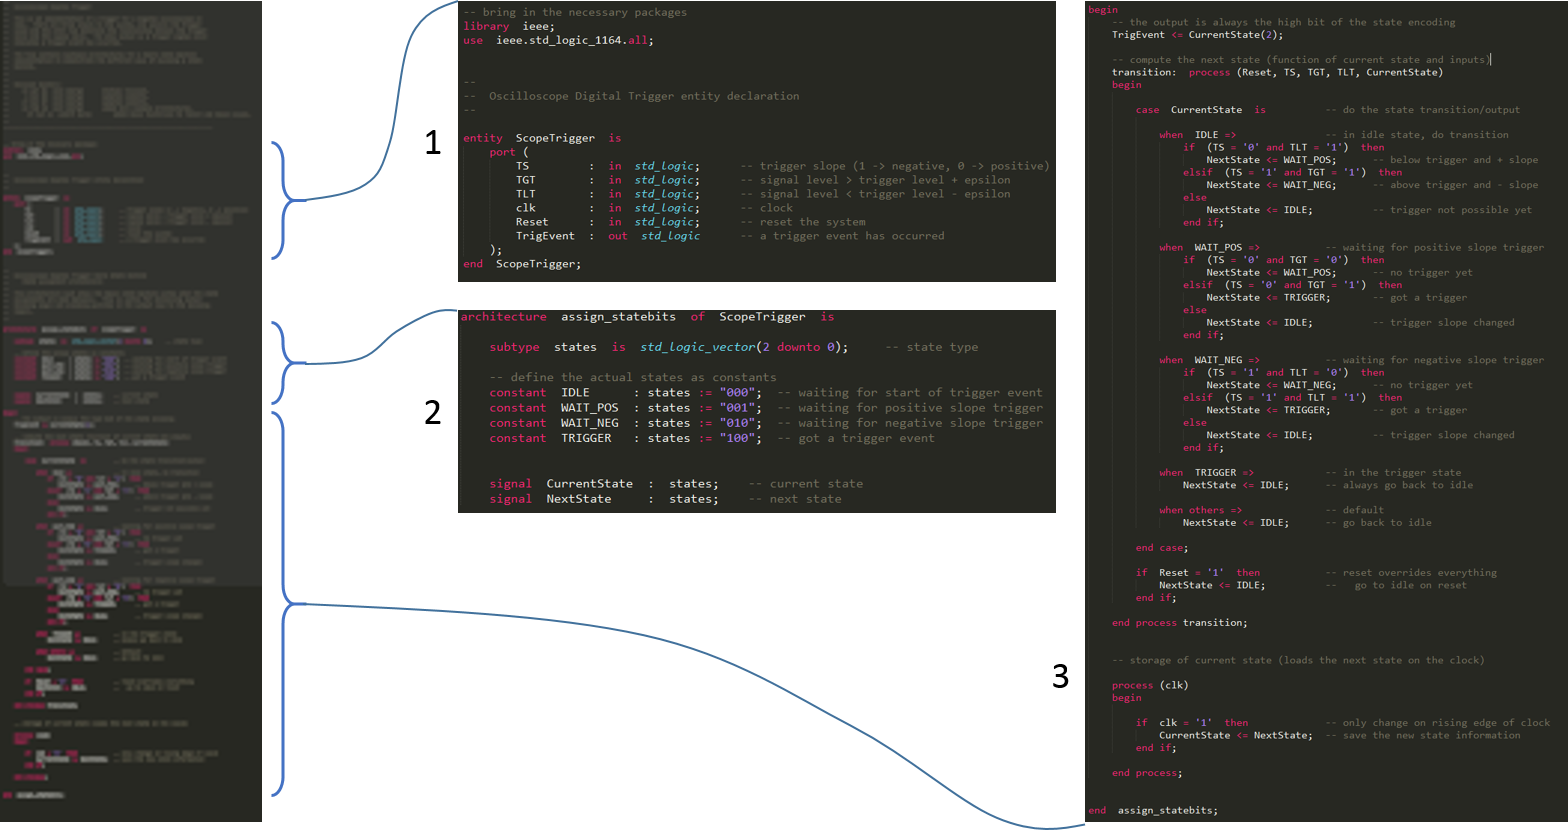
\includegraphics[width=6in]{fpga_logic/vhdl/triggering.png}
		\caption{FPGA triggering state machine}
\end{figure}

Shown above is the trigger state machine. It contains three main components, labeled above as (1) the input and output signals, (2) the states, and (3) the transitions. Operation is fairly straightforward and utilizes hysteresis on the two thresholded inputs. If \verb=TGT= goes from less than to greater than, then the signal just underwent a positive slope transition. The same goes for \verb=TLT= for negative slopes.

Notice that in the \verb=IDLE= state, it can only transition to \verb=WAIT_POS= after going below the lower threshold, whereas the upper threshold is needed to cause a trigger event. This is what allows for hysteresis. The same of course holds for \verb=WAIT_NEG=.

\section{VRAM and Display}

\begin{figure}[ht!]
    \centering
    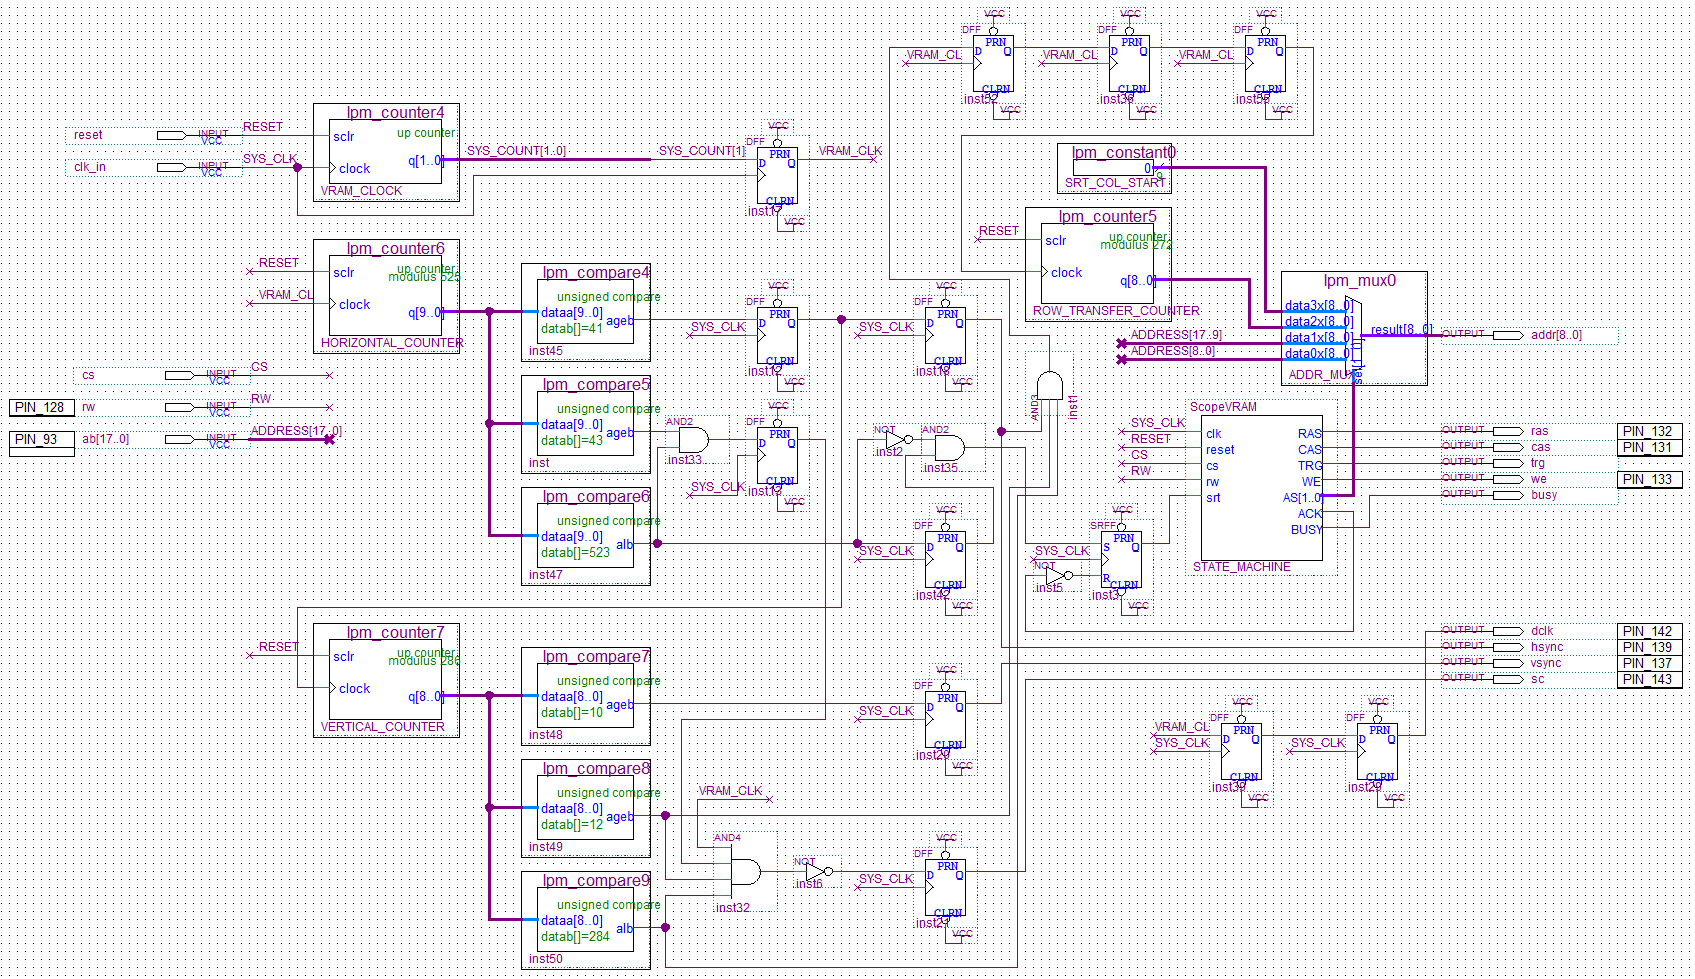
\includegraphics[width=6in]{fpga_logic/vram_disp_overview.png}
		\caption{FPGA overview of VRAM controller and display controller}
\end{figure}

The display and VRAM control logic are lumped together due to the similarities in requirements of their timing (although most of the VRAM control is handled by the state machine). Most of the logic seen above controls timing for the display clocks, while the portion in the upper right is for VRAM control. Much of the VRAM control logic shown here controls the 9-bit VRAM address output.

\subsection{VRAM Controller}

\begin{figure}[ht!]
    \centering
    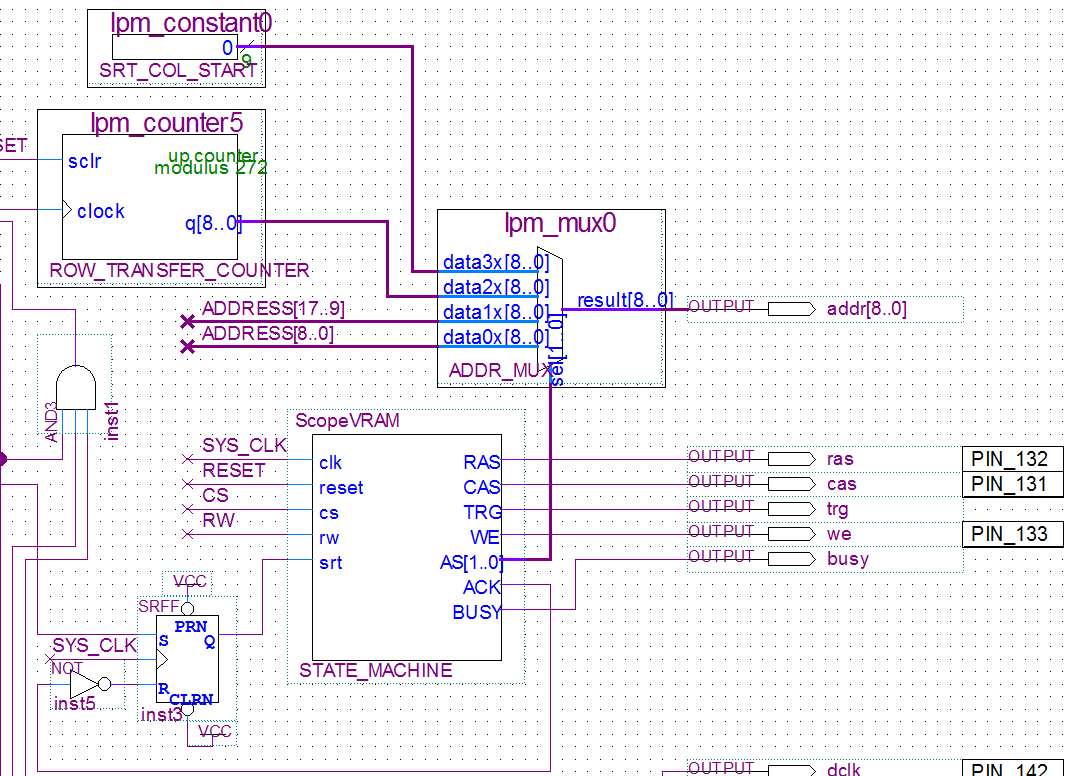
\includegraphics[width=3in]{fpga_logic/vram_disp_addr.png}
		\caption{FPGA VRAM addressing}
\end{figure}

The heart of the VRAM controller is the state machine \verb=ScopeVRAM=. It takes the typical memory outputs of the CPU (CS and RW) and uses that for much more advanced control to the VRAM chip. The state machine only returns a \verb=busy= signal to the CPU to indicate completion of the requested task.

Besides the state machine, the other logic useful for the VRAM controller is selecting the address to put out on the VRAM address bits. This is done by MUXing the two halves of the address bits along with a couple other address, controlled by the state machine. The two halves of the address bus are used for specifying row and column in a standard read to or write from the CPU. The other two address are used for serial row transfer cycles and specify the row (output of \verb=lpm_counter5=) and column to start at (\verb=SRT_COL_START=) for a row transfer. The counter is updated and the serial row transfer state triggered right after every row of pixels is written to the display (at the end of a HSYNC cycle).

\subsection{VRAM State Machine}

\begin{figure}[ht!]
    \centering
    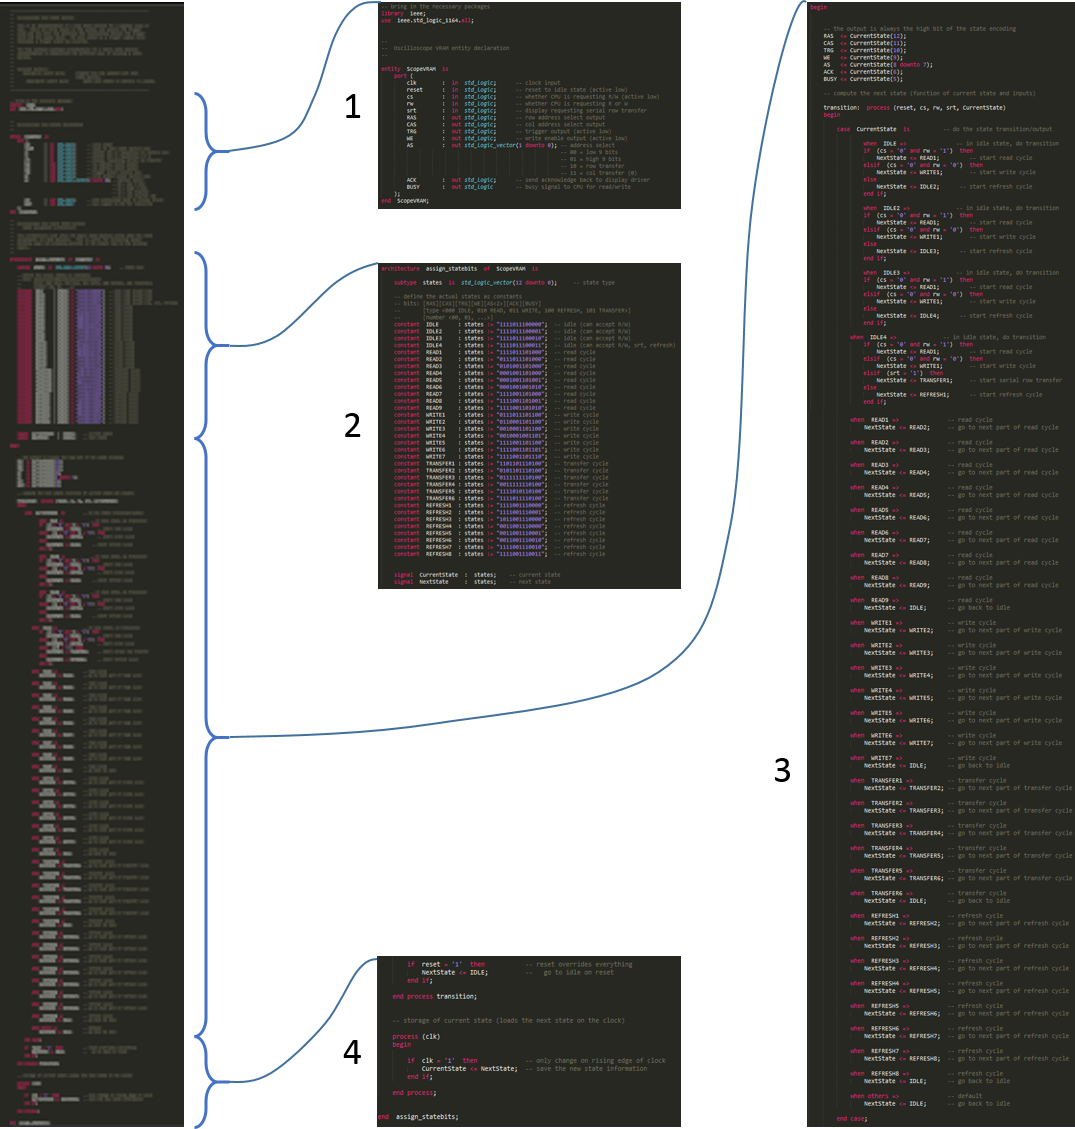
\includegraphics[width=6in]{fpga_logic/vhdl/vstates.png}
		\caption{FPGA VRAM controller state machine}
\end{figure}

The state machine is shown above. Just as in the triggering state machine, the VRAM state machine has (1) the inputs and outputs, (2) the states, and (3/4) the transitions. There are a lot of states, but their purpose is really to handle four main operations: read, write, refresh, and serial row transfer. In any given one of those desired operations, there are a number of states which run sequentially and handle the signal timing for the desired operation. In the transitions (3), you can see that the bulk of transitions move from a state in one operation to the next state in that operation (and at the end going back to \verb=IDLE=).

\subsection{Display Controller}

\begin{figure}[ht!]
    \centering
    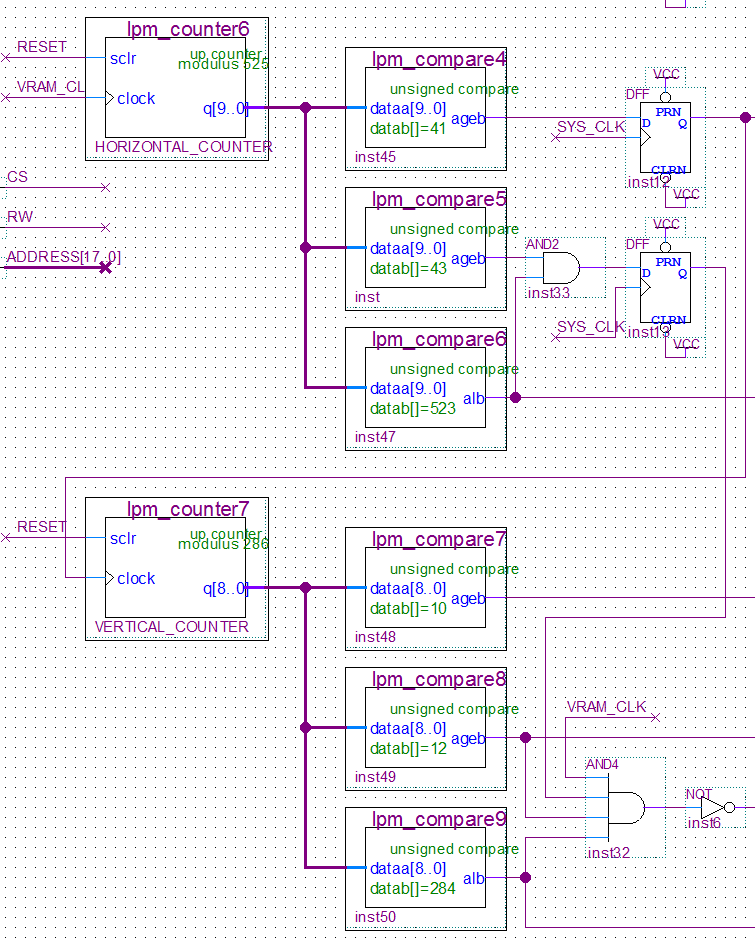
\includegraphics[width=3in]{fpga_logic/vram_disp_counters.png}
		\caption{FPGA display counter timers}
\end{figure}

Display timing is shown above. The \verb=VRAM_CLK= operates at about $9MHz$, approximately the dot clock frequency required by the display. \verb=lpm_compare4-6= then take care of a given HSYNC cycle - mainly the HSYNC pulse and the back and front porches. The HSYNC pulse in turn acts as a clock for the VSYNC counter. \verb=lpm_compare7-9= take care of a given VSYNC cycle - mainly the VSYNC pulse and the back and front porches.

\subsection{Display Timing (Testing)}

The tough timing requirements make testing a very good idea. Testing was done in Altera ModelSim with VHDL test code (provided in the appendix). To prove the importance of testing, here's an initial run of the display timing.

\begin{figure}[ht!]
    \centering
    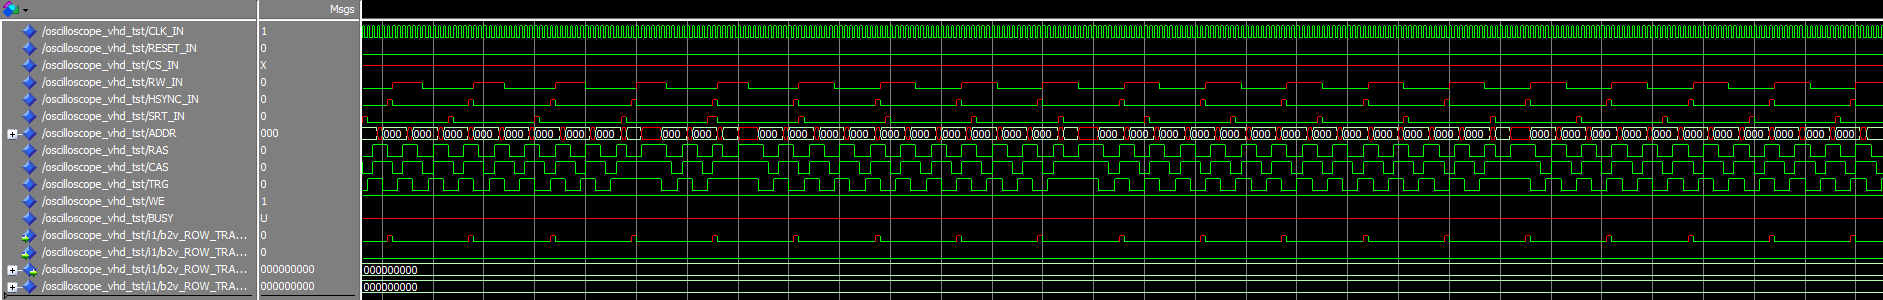
\includegraphics[width=4in]{timing/VRAM-test/vram-problem-start.png}
		\caption{Display timing test, problematic start}
\end{figure}

Notice that large portions of the signal are red, indicating there's a timing problem. In contrast, a successful run should have all green signals. Shown below is a semi-successful startup. The signals start out red due to a conflict in signal outputs (this was fixed), but then everything works properly.

\begin{figure}[ht!]
    \centering
    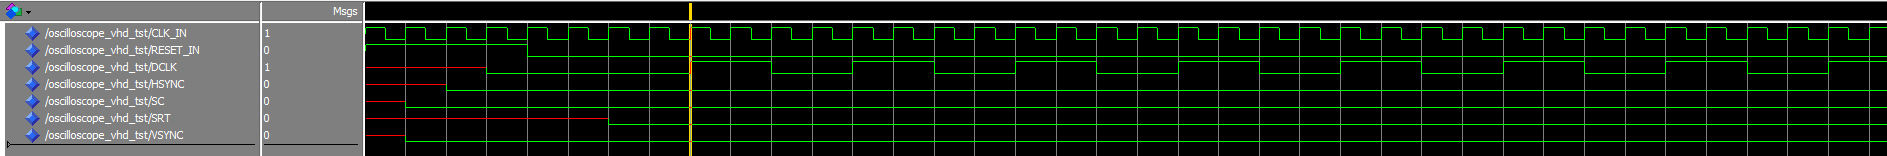
\includegraphics[width=6in]{timing/VRAM-test/display-success-start.png}
		\caption{Display timing test, semi-successful start}
\end{figure}

After fixing everything, all of the timing works out properly. Here are the signals at different zoom levels. First, looking at just the pulse of a horizontal cycle. Then looking at the full horizontal cycle. Then, looking at a pulse of a vertical cycle, and finally the full cycle (each period represents one full display refresh).

\begin{figure}[ht!]
    \centering
    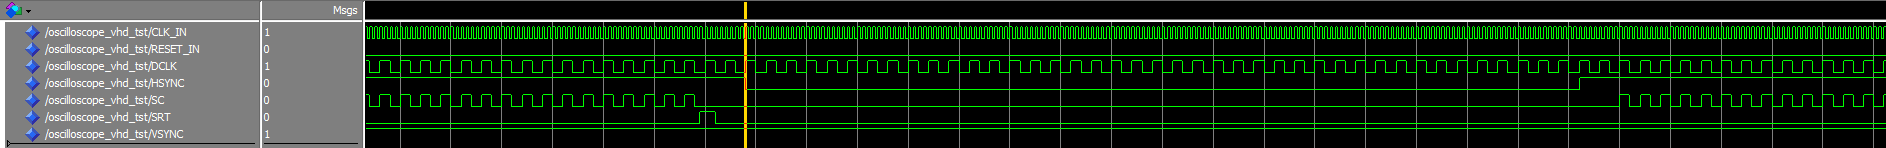
\includegraphics[width=6in]{timing/VRAM-test/display-success-horiz-pulse.png}
		\caption{Display timing test, successful horizontal pulse}
\end{figure}

\begin{figure}[ht!]
    \centering
    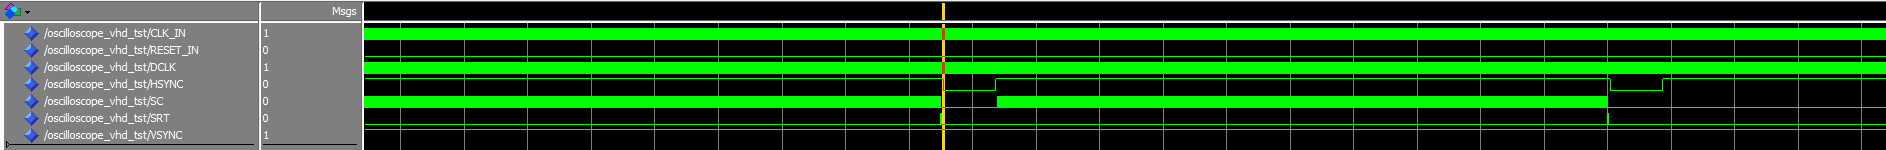
\includegraphics[width=6in]{timing/VRAM-test/display-success-full-horiz.png}
		\caption{Display timing test, successful horizontal cycle}
\end{figure}

\begin{figure}[ht!]
    \centering
    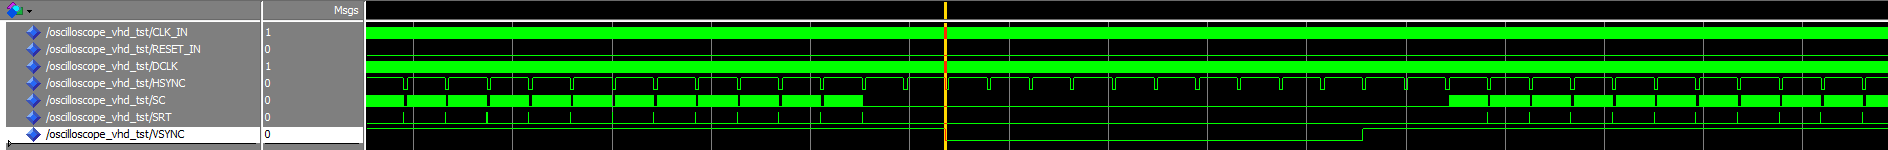
\includegraphics[width=6in]{timing/VRAM-test/display-success-vert-pulse.png}
		\caption{Display timing test, successful vertical pulse}
\end{figure}

\begin{figure}[ht!]
    \centering
    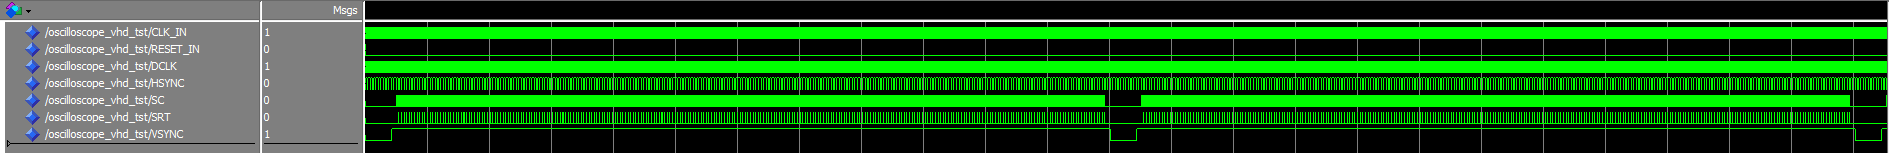
\includegraphics[width=6in]{timing/VRAM-test/display-success-full-vert.png}
		\caption{Display timing test, successful vertical cycle}
\end{figure}

We can see that the results are successful:

\begin{figure}[ht!]
    \centering
    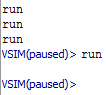
\includegraphics[width=1in]{timing/VRAM-test/display-success-full-output.png}
		\caption{Display timing test, all tests successful}
\end{figure}

\section{Switches}

All of the switch debouncing and decoding is done in FPGA logic. All of the switch-handling logic is shown here:

\begin{figure}[ht!]
    \centering
    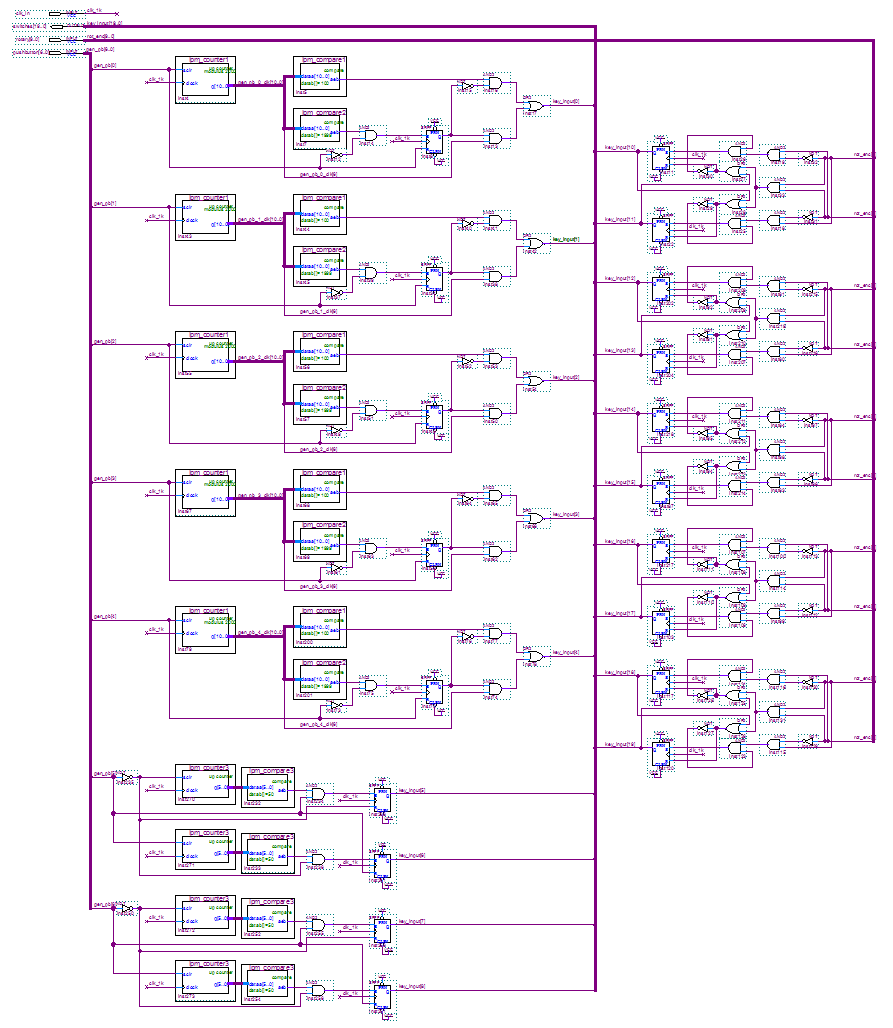
\includegraphics[width=6in]{fpga_logic/keys_overview.png}
		\caption{FPGA overview of key and rotary encoder input}
\end{figure}

The five display buttons are handled by logic in the top left, the two latching pushbuttons are handled in the bottom left, and the rotary decoding is handled by the five circuits on the right.

\subsection{Momentary Pushbutton Input}

The following logic circuit shows how the more basic momentary pushbuttons are debounced. When a pushbutton signal (active low) comes in, it unsets the counter clear, which allows the counter to start incrementing. If the button is pressed long enough without a bounce, then the counter will reach the first compare value, generating an interrupt for the CPU. If the switch continues being pressed, the second compare also kicks in and handles automatic switch repetition.

\begin{figure}[ht!]
    \centering
    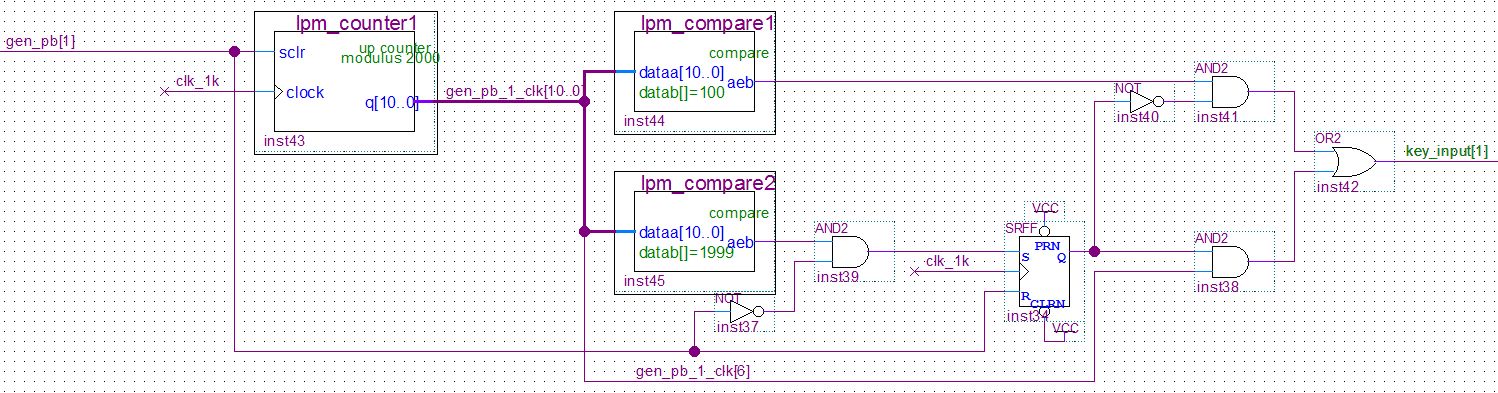
\includegraphics[width=6in]{fpga_logic/keys_pb.png}
		\caption{FPGA momentary pushbutton input debouncing}
\end{figure}

\subsection{Latching Pushbutton Input}

The latching pushbuttons are debounced in a similar manner to the momentary ones, with a counter/compare pair. However, there's no need for switch repetition. Instead, there's a need for debouncing the switch in both directions (hence the pair of counter/compares). Closing the pushbutton as well as openning the pushbutton will send separate interrupts to the CPU.

\begin{figure}[ht!]
    \centering
    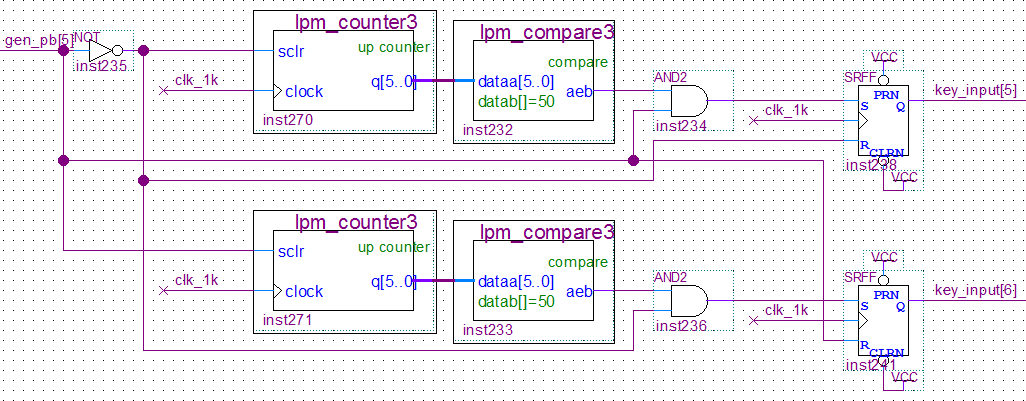
\includegraphics[width=6in]{fpga_logic/keys_pb_latching.png}
		\caption{FPGA latching pushbutton input debouncing}
\end{figure}

\subsection{Rotary Encoder Input}

At each detent of the rotary encoder, the A and B lines are held high. During a rotation by one detent, the A and B lines cycle through a grey code pattern depending on which direction the rotation was in. We can see this pattern in the diagram below. One way we can decode the signal, then, is to detect which of $\{A,B\}$ lines go low first (this indicates the rotation direction), and then wait for both of them to return high before going back to the initial state.

The diagram below shows the exact opposite polarity as what's described above, but the function is exactly the same.

\begin{figure}[ht!]
    \centering
    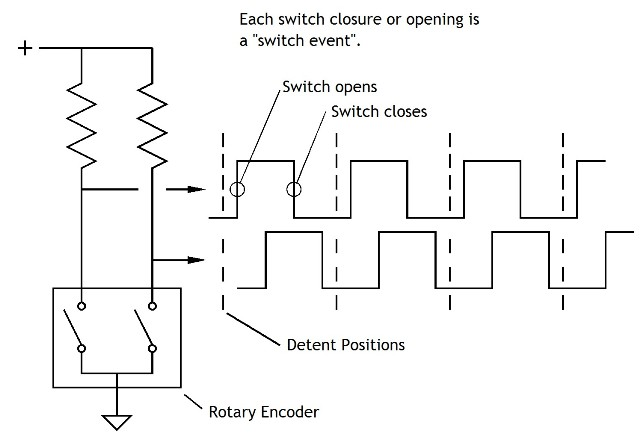
\includegraphics[width=3in]{Timing/encoder.jpg}
		\caption{Rotary encoder timing}
\end{figure}

We see that logic in the following circuit. In this circuit, the A and B rotary encoder lines come in from the right, and then interrupts for each of a CW or CCW turn are sent to the CPU on the left. We see the actual logic as described above. Whichever line falls low first sets the appropriate SRFF (triggering either a CW or CCW interrupt), and suppresses the other line from setting the opposing SRFF. Finally, the reset signal is generated when both lines go high again.

\begin{figure}[ht!]
    \centering
    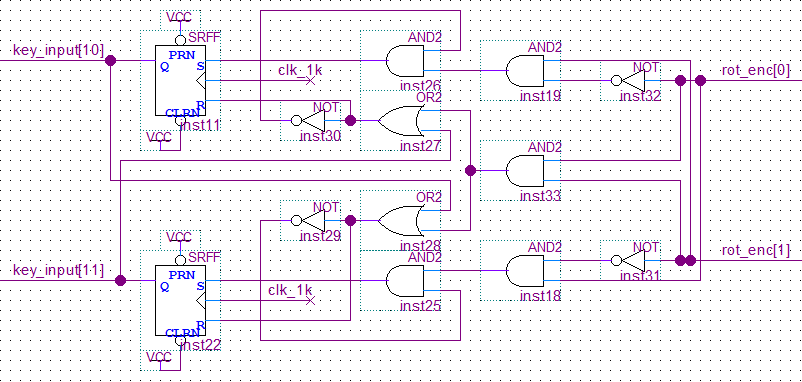
\includegraphics[width=6in]{fpga_logic/keys_rotary.png}
		\caption{FPGA rotary encoder decoding}
\end{figure}

\newpage
\section{NIOS II Processor}

\begin{figure}[ht!]
    \centering
    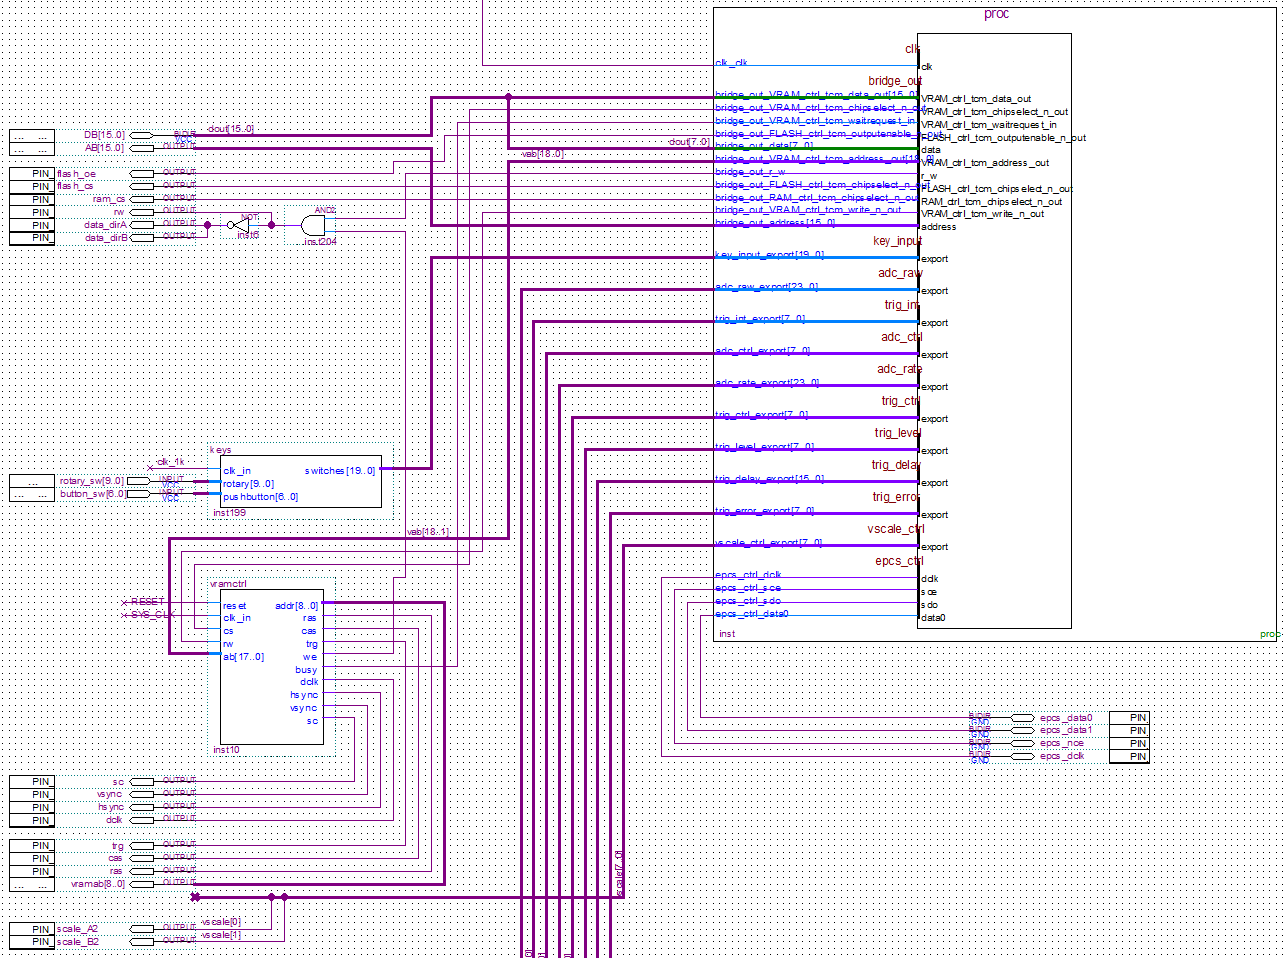
\includegraphics[width=6in]{fpga_logic/proc_overview.png}
		\caption{FPGA NIOS II processor block}
\end{figure}

The Altera Cyclone III FPGAs have enough logic gates to support a simple processor, called the NIOS II. It has a RISC architecture with 32 registers and a small instruction set. More information about the NIOS II can be found online.

In the circuit above, the processor and some core peripherals are shown in a single block at the top right. It interfaces with FPGA I/O (at the left of the schematic), as well as the key and VRAM control modules (middle left), EPCS (bottom right), and triggering logic (not shown, below).

\subsection{Overview of Capabilities}
\begin{figure}[ht!]
    \centering
    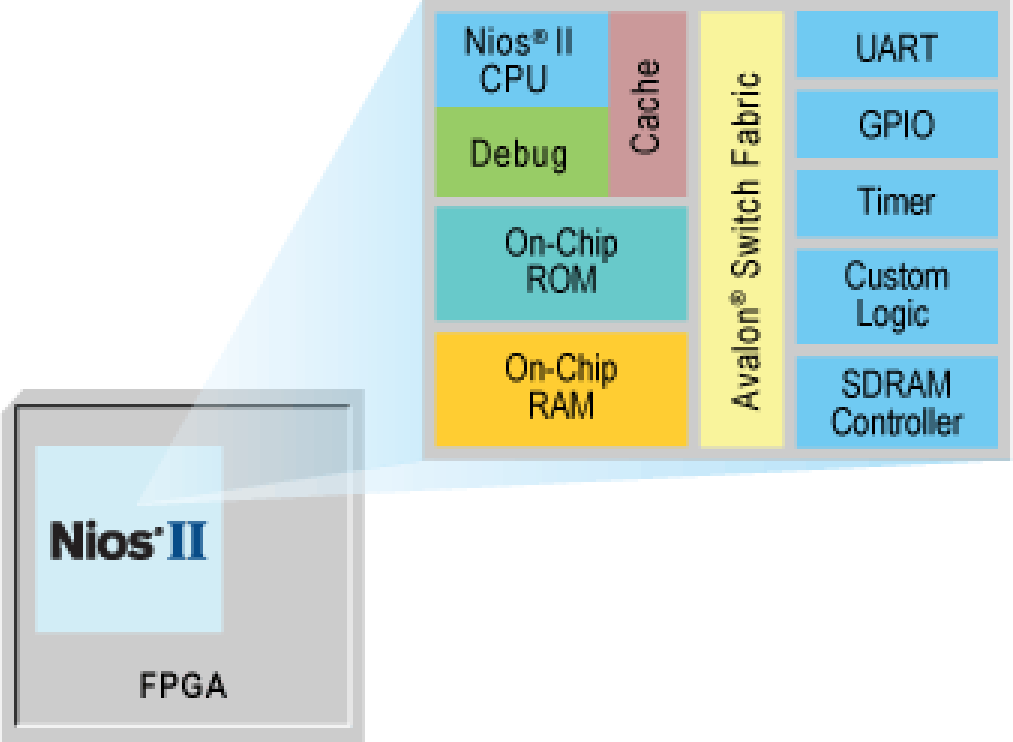
\includegraphics[width=2in]{images/nios_ii.png}
		\caption{NIOS II soft core processor}
\end{figure}

The processor can be built up using the a subtool of Quartus called QSYS. This system can be used to create not only the core NIOS processor, but also supporting components such as an Avalon bus for managing peripherals, interrupts, input and output to the CPU, etc.

Once the processor is designed in QSYS, it can be generated into a block for use in the logic circuit. In a block diagram file, all inputs/outputs exported in the QSYS screen can be hooked up directly to the other FPGA logic. This allows for seamless integration of the FPGA logic and the soft core CPU.

\subsection{Peripherals}

In addition to the basic NIOS II processor and clock, there are a number of peripherals we can add.

For memory modules which share signals to the outside world, we do this with a Generic Tri-State Controller for each memory module, a Tri-State Conduit Pin Sharer to share certain connections/buses, and finally a Tri-State Conduit Bridge takes the shared symbols and exports them as pins on the processor block.

For simple inputs/outputs between the processor and the outside world, a simple Parallel I/O peripheral can be used. These PIOs can be configured as input, output, and bidirectional. Inputs can trigger interrupts.

\begin{figure}[ht!]
    \centering
    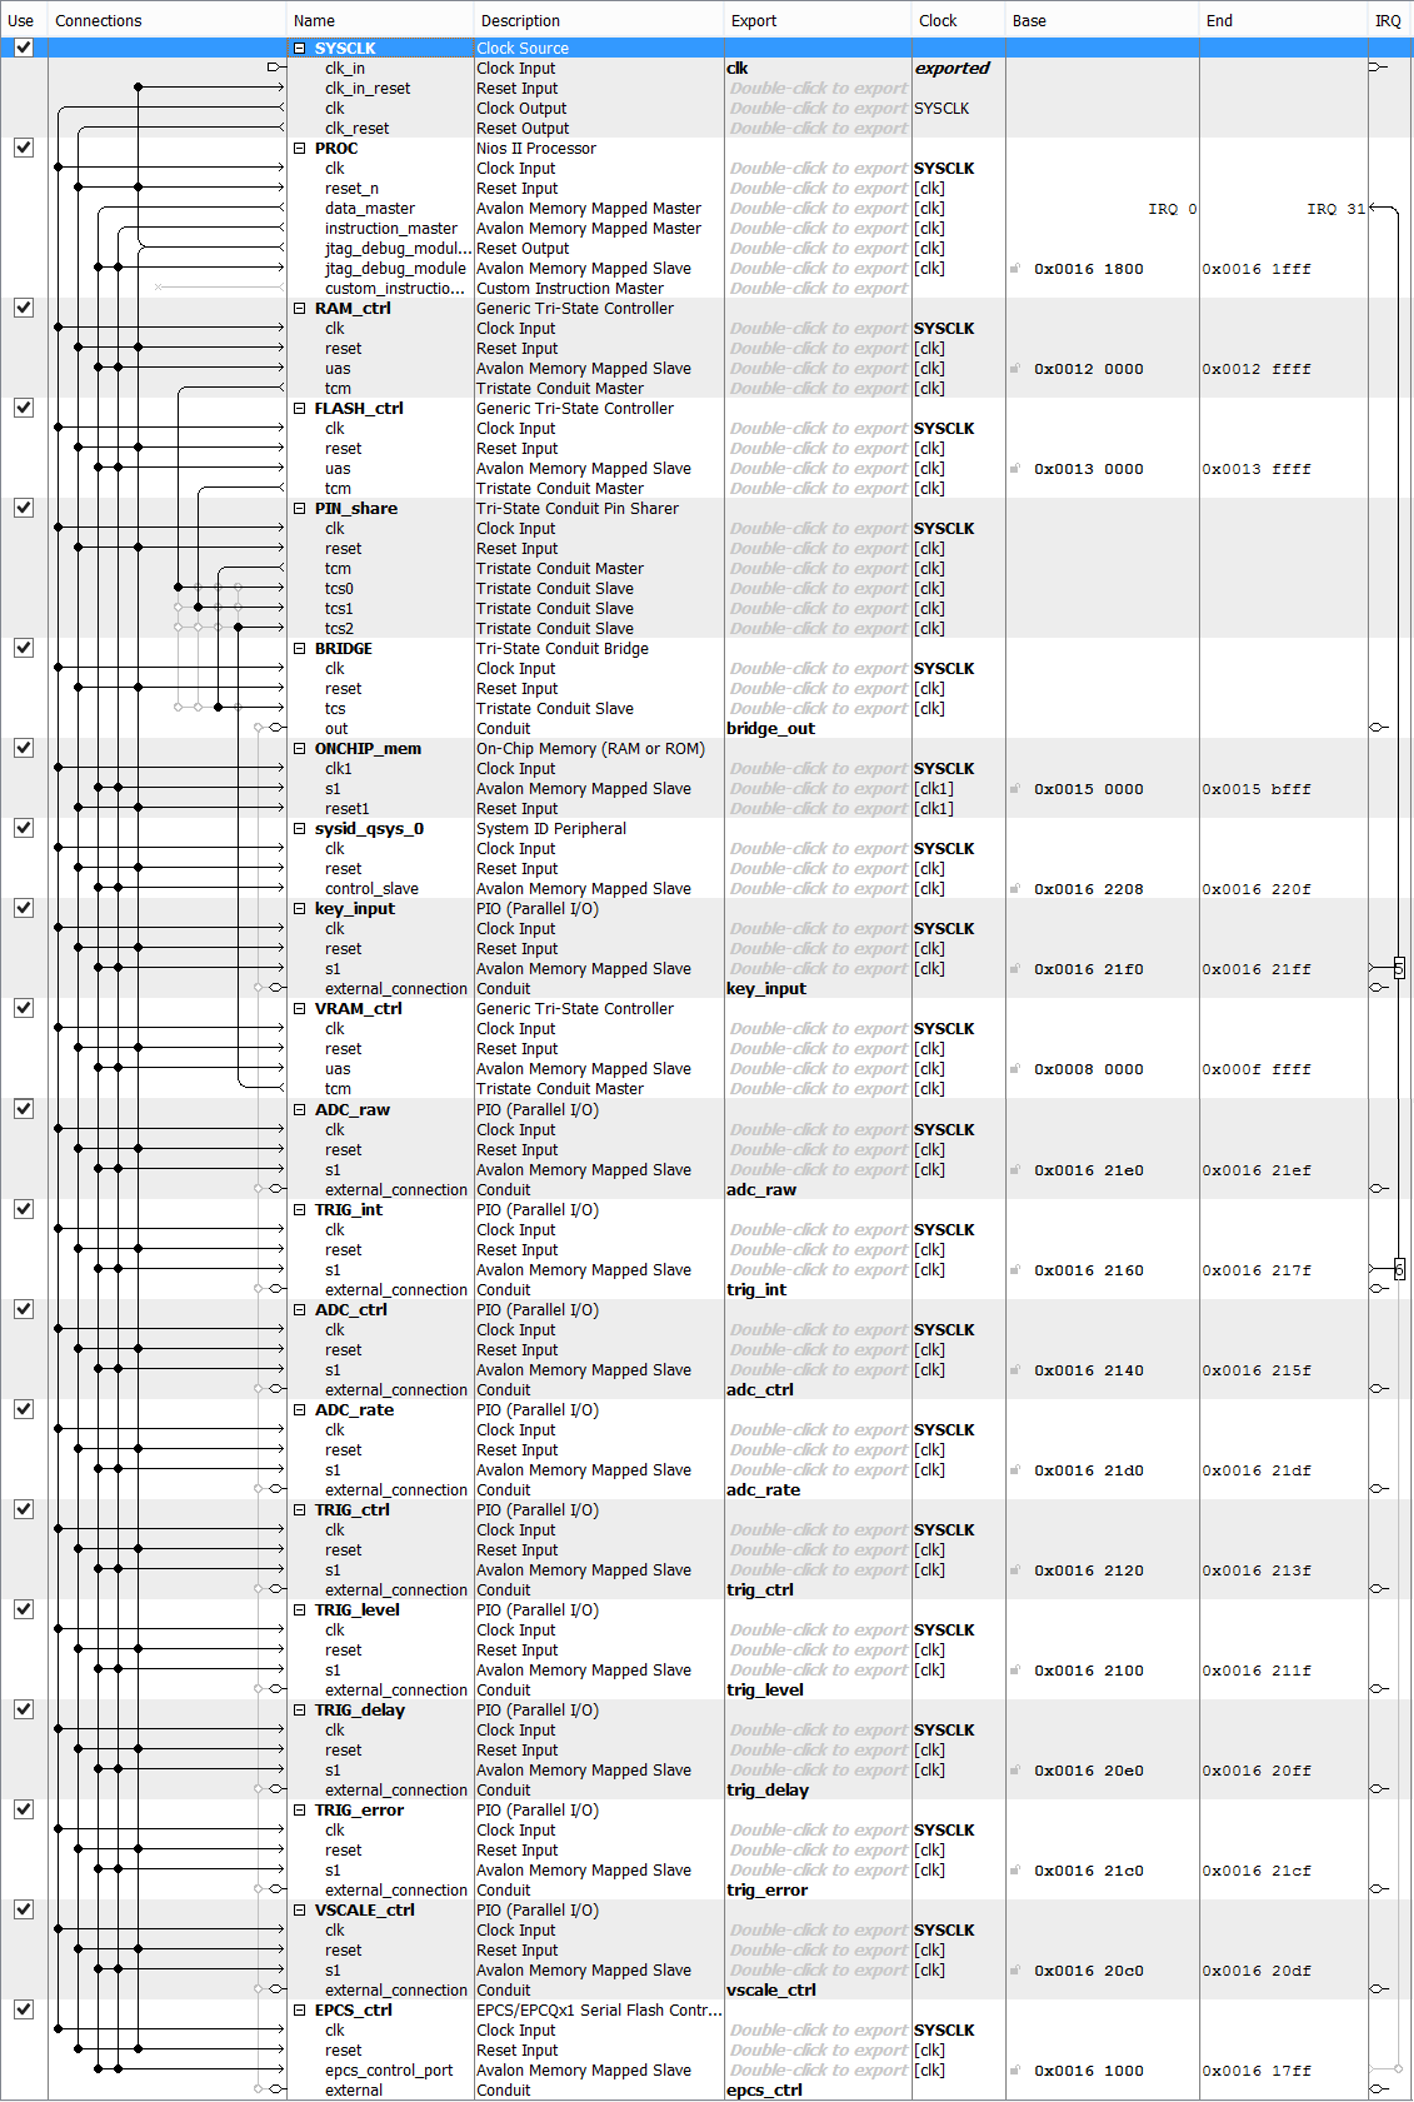
\includegraphics[width=4in]{fpga_logic/proc_periph.png}
		\caption{NIOS II core peripherals}
\end{figure}

\subsection{NIOS II Settings}

These are the settings for the NIOS II processor. We're using the NIOS II/s version, which includes instruction caching and hardware divides. Caching is particularly important. Without caching, the processor runs much slower and the LCD refresh rate is very noticeable.

\begin{figure}[ht!]
    \centering
    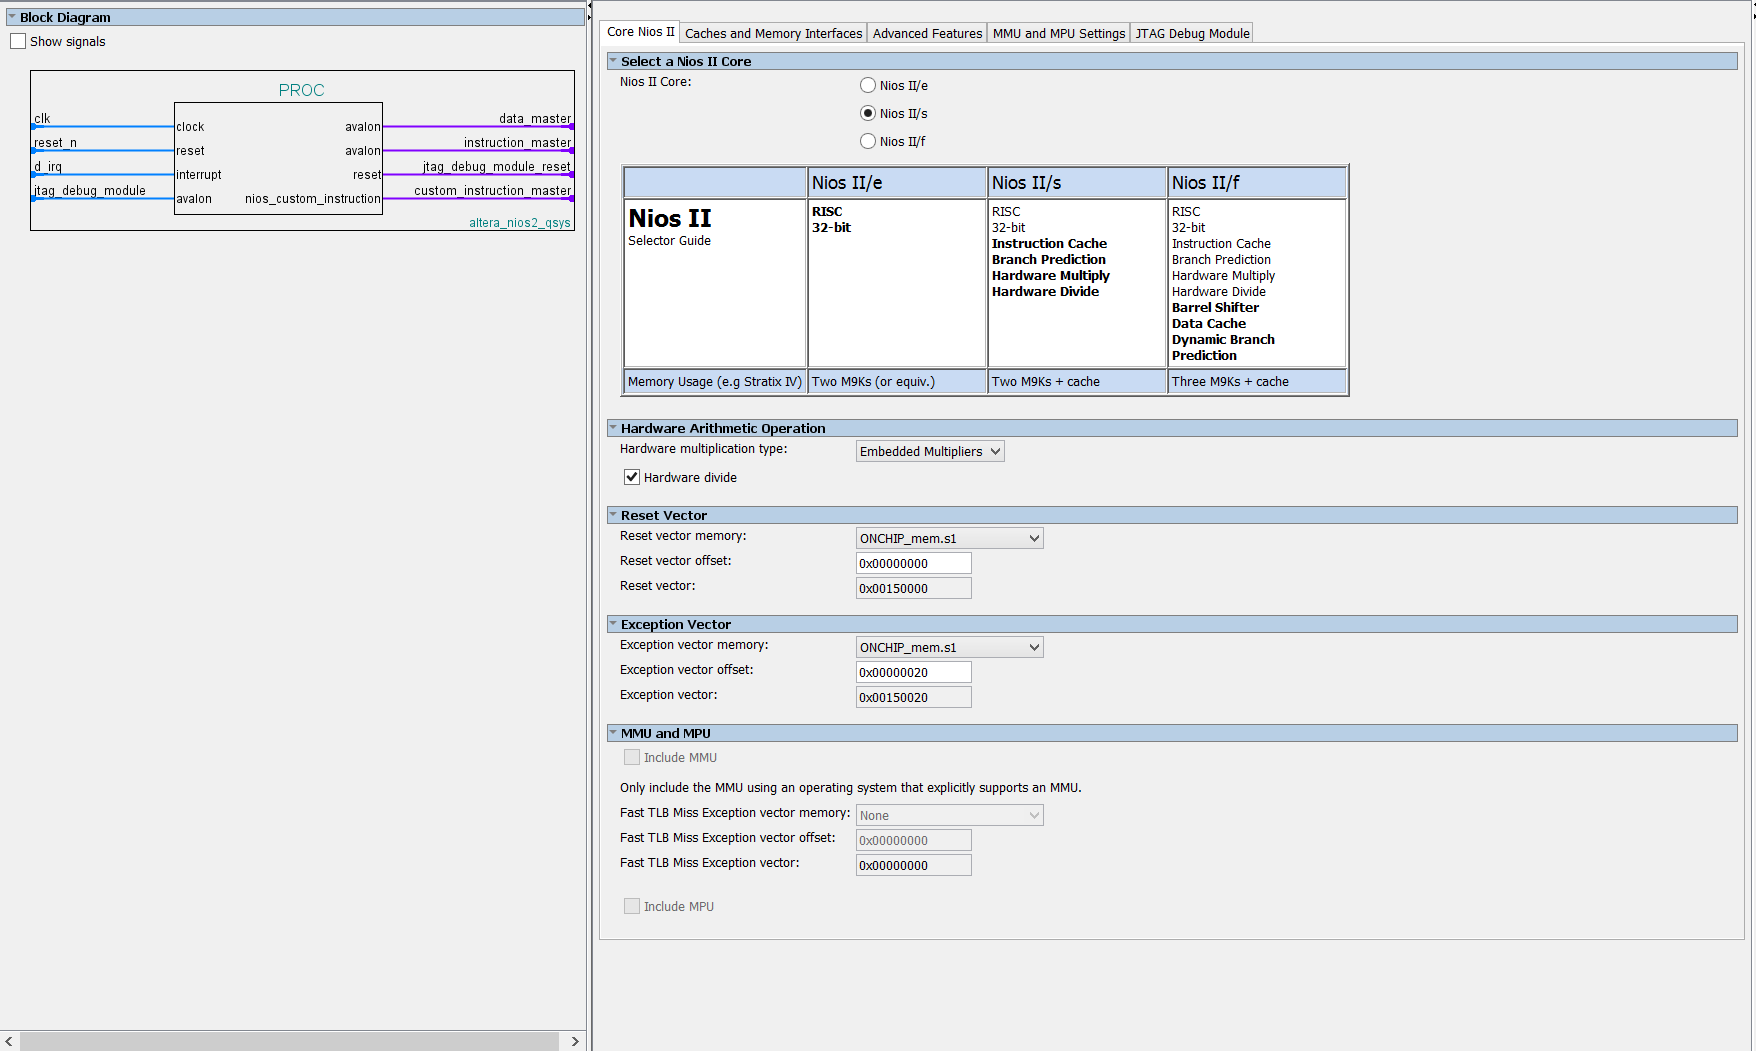
\includegraphics[width=4in]{fpga_logic/proc_settings.png}
		\caption{NIOS II core settings}
\end{figure}

\subsection{Address Memory Map}

Finally, with this whole QSYS processor setup, we can generate the addresses for each component, seen below. Once that's done, we generate the entire processor (VHDL file, as well as a block diagram block). Configuration details about the base addresses (including \verb=#define=s) of each of these peripherals is included in the generated processor files. This can be used in the NIOS II code to allow for easy maintenance of the NIOS code, agnostic to changes in the actual base addresses.

\begin{figure}[ht!]
    \centering
    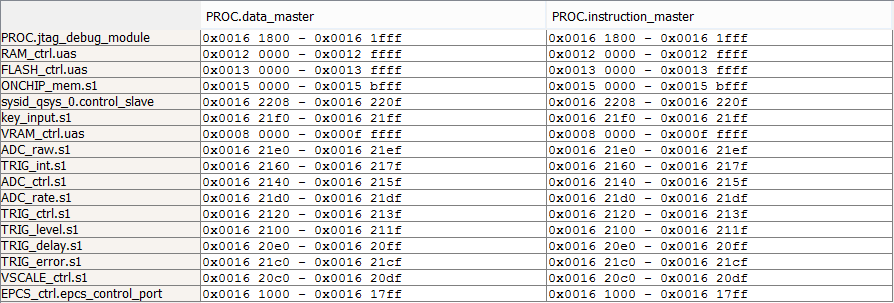
\includegraphics[width=6in]{fpga_logic/address_map.png}
		\caption{NIOS II address memory map}
\end{figure}
